% !TEX root = ../thesis.tex
% sensor-array prinziple
% @author Tobias Wulf
%

\section{Prinzip des Sensor-Arrays}\label{sec:prinzip-des-sensor-arrays}
\begin{itemize}
	\item geometrischer Aufbau
	\item Brückenausgangsspannungen
	\item Resultierende Array-Datenformate und Darstellung der Sinoiden
\end{itemize}


\begin{figure}[tbph]
	\centering
	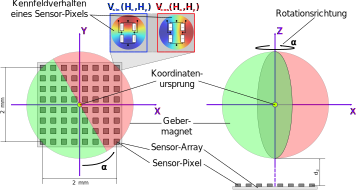
\includegraphics[width=.9\linewidth]{chapters/images/2-Grundlagen/Sensor-Array-Prinzip}
	\caption[Geometrischer Aufbau und Ausrichtung des Sensor-Arrays]{Geometrischer Aufbau und Ausrichtung des Sensor-Arrays. Quadratische Anordnung von Sensor-Pixeln zu einem $8 \times 8$ Sensor-Array. Alle Pixel sind gleich verteilt auf der Array-Fläche. Sensor-Pixel-Verhalten ist aus Kennfeldern entnommen und ortsabhängig von Pixel-Position im Koordinatensystem. Array-Kantenlängen sind mittig von Eck-Pixel zu Eck-Pixel bestimmt. Ebenfalls der $Z$-Abstand zur Magnetoberfläche. Abstände innerhalb der Pixel sind vernachlässigt. Das Array ist zentriert in der $Z$-Achse ausgerichtet. Ideal lotrecht zur Nord-Süd-Ausrichtung des Magneten. Koordinatenursprung des Gesamtsystem liegt in der Gebermagnetmitte. Gebermagnet ist ein Kugelmagnet, der um seine $Z$-Achse rotiert. Grafik nachempfunden und bearbeitet aus \cite{Schuethe2020b}.}
	\label{fig:sensor-array-prinzip}
\end{figure}


\begin{figure}[tbph]
	\centering
	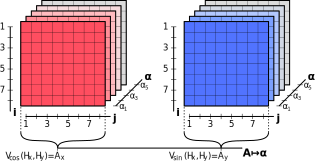
\includegraphics[width=0.9\linewidth]{chapters/images/2-Grundlagen/Sensor-Array-Daten}
	\caption[Resultierende Sensor-Array-Daten]{Resultierende Sensor-Array-Daten}
	\label{fig:sensor-array-daten}
\end{figure}

\clearpage